\documentclass[12pt,letterpaper]{book} % a4paper
   
% packages
\usepackage{graphicx}
\usepackage{hyperref}
\usepackage{pdfpages}

% variables
\newcommand{\picSize}{0.19\textwidth}
\newcommand{\textSize}{0.79\textwidth}

% define the title
\title{Open Data Lab Annual Report: FY19-20}
\author{The Open Data Lab Collaboration}

%%% ---ooo000 END PREAMBLE 000ooo---

\begin{document}
\pagestyle{headings}
% generates the title

\frontmatter
\cleardoublepage
\maketitle

\cleardoublepage
\begin{figure}[!hbtp]
\includegraphics[width=\textwidth]{cover-images/ODLFrontCover-nontrans}
\end{figure}

\newpage

%\pagestyle{plain}
%\thispagesytle{plain}


\begin{tabular}[t]{lp{\textSize}}
\hline
\hline
%\includegraphics[width=\picSize,trim=0 0 0 -0.1\textwidth]{images/people/alonzi.png} 
\raisebox{-0.9\totalheight}{\includegraphics[width=\picSize]{images/people/alonzi.png}}
& 
\begin{tabular}[t]{p{\textSize}}
"At vero eos et accusamus et iusto odio dignissimos ducimus qui blanditiis praesentium voluptatum deleniti atque corrupti quos dolores et quas molestias excuri sint occaecati cupiditate non provident,At vero eos et accusamus et dent, " 
\end{tabular}
\\
\rule{0pt}{0.2\textwidth} & \rule{0pt}{0.2\textwidth} \\
\hline
\rule{0pt}{0.2\textwidth}
\includegraphics[width=\picSize]{images/people/bourne.png}
 & text \\
\hline
\rule{0pt}{0.2\textwidth}\includegraphics[width=\picSize]{images/people/clark.png} & text \\
\hline
\rule{0pt}{0.2\textwidth}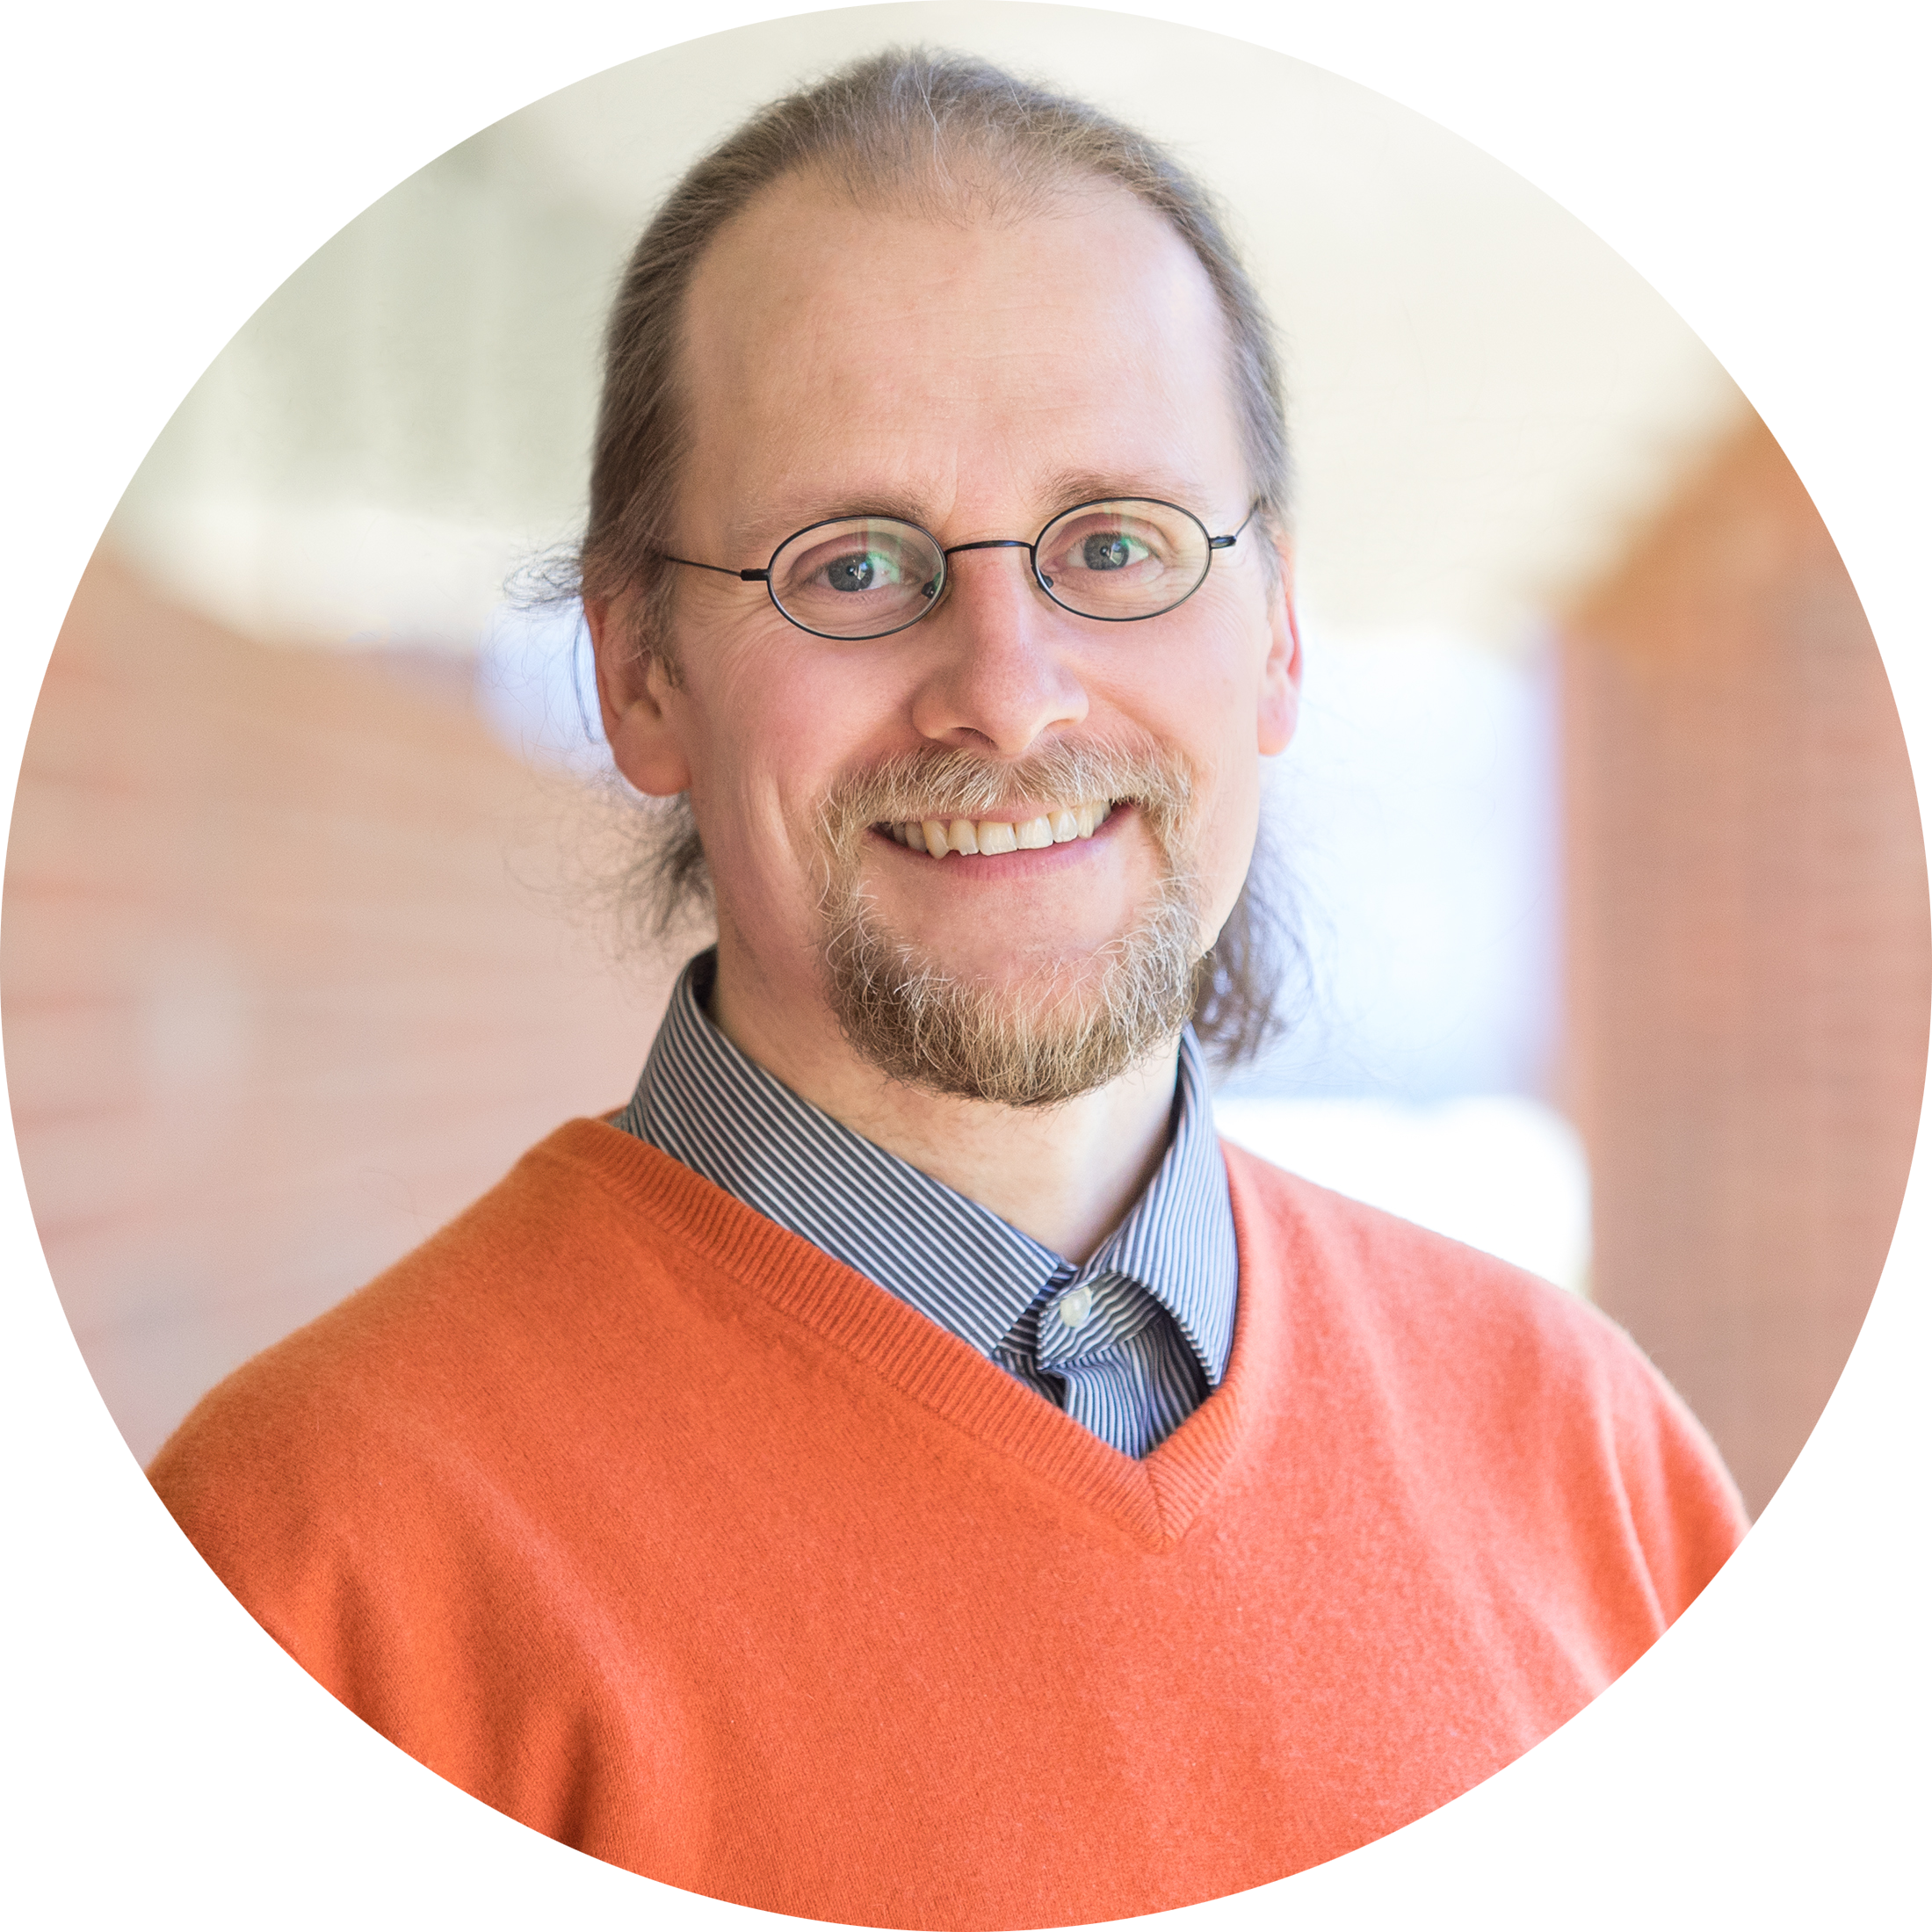
\includegraphics[width=\picSize]{images/people/mietchen.png} & text \\
\hline
\rule{0pt}{0.2\textwidth}\includegraphics[width=\picSize]{images/people/rasberry.png} & text \\
\hline
\hline
\end{tabular}

% \smash{...} to override bounding
 % People working on project, alphabetical
\chapter{Project manager's note}  At the beginning of 2018 the Open Data Lab was an idea, a sketch on a whiteboard. Today the Open Data Lab has over 100 users. Students at the University of Virginia have used it to conduct research published by IEEE. In just over a year a small team of dedicated individuals from the Data Science Institute at UVA produced a product that furthered the educational and research mission of the University. Today students at UVA can do things they could not do before this project launched.

I am extremely honored to have been asked to lead this effort. The work done by our collaboration is of the very best calibre and I am proud of the work we have done and will do in the future. As project manager I feel I have the easiest job on the team. I ask everyone for ideas and they put forth not just an enormous number of ideas but also brilliant ideas. The hardest part for me is to choose from all the great ideas. Without the team Phil Bourne has built my job would be impossible. With this team I do not see any limit to what we can achieve.

The first year of the Open Data Lab was one of exploration. We discovered new tools, in particular the value of Project Jupyter. We also interviewed our potential users and recognized archetypes which we can use to guide what we build. Putting all of this together we are currently developing a strategic plan for the next three years. We now look to make an impact in the community and I am excited for what is to come.

\begin{flushright}

\bigskip

Open Data Lab Project Manager

\bigskip

Peter Alonzi

\end{flushright}
 % Mission and vision and philosophy
\chapter{Executive Briefing}The 2018-2019 year was the first year for the Open Data Lab. In this time we learned many things and many users attended workshops, hosted and anlyzed data, some event produced a publication. We served 116 users, working on 25 projects, and 6 individuals contributed directly to the ODL project. Going forward we look to increase all of those numbers including users from beyond the Data Science Institute.

Here are a few highlights from 2018-2019:
\begin{itemize}
\item Development of a GitHub workflow for beginners useful beyond the hard sciences. This workflow was adopted by an international collaboration called the Open Greek and Latin Project~\cite{ref:oglp} as well as the Archaeology Department of Monticello~\cite{ref:tjf}. Details are found on our github page and in Section~\ref{sec:git}.
\item We realized the power of Project Jupyter as a system to deliver resources to the user without excessive cognitive load. This platform is transformative and will lead to great things in the future. Details are found in Section~\ref{sec:projectjupyter}.
\item We studied three user archetypes for the Open Data Lab: the collaborator, the student, and the sharer. Details are round in Section~\ref{sec:archetypes}.
\end{itemize}

We have accomplished a lot but now we need help. If you have an idea or want to join the team please reach out by emailing datascientist@virginia.edu (Subject Line: "I want to help the ODL").

% \footnote{https://www.dh.uni-leipzig.de/wo/projects/open-greek-and-latin-project/}
% \footnote{https://www.monticello.org/site/research-and-collections/monticello-archaeology}
% insert the table of contents
\chapter*{Bug Bounty Program}
We encourage close reading and critique of the Open Data Lab proceedings. If you find a bug in any of our work including this report please let us know. The best way to pass along notes is through a pull request on our github page: \url{https://github.com/UVA-DSI/Open-Data-Lab}.

\tableofcontents
\listoffigures
\listoftables

\mainmatter
\chapter{Overview} \section{What is the Open Data Lab?}
\subsection*{OPEN}
We encourage all users to be as open as possible with every aspect of their work. That may be in opening up their data sets, publication, source code, or ...
\subsection*{DATA}
We take an expansive definition of data. Everything from traditional data, to code, to workflows, to published material, and so on is considered data to us. We provide a place for all things digital data.
\subsection*{LAB}
We provide a place where the power of contemporary computing can be brought to bear against data resources. Given the scale of data today this means colocating the data and computational resources.
\subsection*{Open Data Lab}
The Open Data Lab is a resource to provide state of the art computing and data infrastructure to researchers, students, and sharers. It is guided by the principles of science and openness.
 
\section{User Archetypes}
There are many potential use cases for the Open Data Lab. In this section we describe the three cases that have been tested so far. They are: the Collaborator, someone who is working on a research project; the Student, someone who is using the Open Data Lab to learn about data science; and the Sharer, a person with data who wants to open it up to a broader audience.

\subsection*{The Collaborator}
This archetypal person uses the Open Data Lab to conduct research. They access data and computational resources that are colocated. This colocation facilitates lower latency and increased performance. A wide range of services can be provided globally by AWS and locally through UVA HPC resources. Sample workflow:
\begin{enumerate}
\item Request a user account on the Open Data Lab
\item Once per collaboration:
\begin{enumerate}
\item Load data 
\item Provision computational resources
\end{enumerate}
\item Conduct research operations
\item Register resulting products in Dataverse
\end{enumerate}

\subsection*{The Student}
This archetype uses the Open Data Lab to facilitate learning. An example would be someone who participates in a workshop where and ODL notebook instance powered by AWS SageMaker provides the working environment. Sample workflow:
\begin{enumerate}
\item Request a user account on the Open Data Lab
\item Logon to AWS console to launch Jupyter
\item Use Jupyter during the workshop
\end{enumerate}

\subsection*{The Sharer}
This archetype is a user who owns data and wants to make it available. There are many mechanisms for sharing the data ranging from RESTful API of S3, to a SPARQL endpoint. Sample workflow:
\begin{enumerate}
\item Request a user account on the Open Data Lab
\item Load data into an S3 bucket
\item Configure one of the following
\begin{enumerate}
\item SPARQL endpoint
\item API Gateway to access S3
\item S3 permissions for a SageMaker notebook
\item ...
\end{enumerate}
\end{enumerate}

\section{User Summary}
\begin{center}
\begin{tabular}{lccr}
\hline
\hline
group & projectID & \# members & type \\
\hline
\hline
Bourne-Mura & bamc & 4 & MSDS Capstone \\
CBW & cbwc & 4 & MSDS Capstone\\
Wiki & wiki & 9 & MSDS Capstone\\
Mental Health & miip & 6 & SYS Capstone\\
\hline
Women Terror Recruitment & watr & 2 & Presidential Fellow\\
\hline
Healthy Markets & hmtt & 5 & DSI Research\\
Independent Study & pmis & 1 & DSI Research\\
\hline
Linked Open Data   & nept & 2 & External Data\\
\hline
Spark & sprk & 17 & Education \\
GitHub & gith & 9 & Education \\
\hline
ORCI & orci & 2 & ODL Development\\
\hline
ML under & mlunder & 7 & Club\\
ML grad & mlgrad & 3 & Club\\
\hline
Rivanna & -- & 11 & Local\\
Ivy & -- & 6 & Local\\
\hline
\hline
ODL-education  & -- & 26 & Education Users\\
ODL-users & -- & 68 & Unique Users\\
\hline
\hline
\end{tabular}
\end{center}

\section{A phased approach}
\label{phases}
The first three phases of the Open Data Lab have been outlined. Phase 0 focused on pre investigation and decided on what technology to test in Phase 1, the closed beta. Phase 2 is an open Beta and will serve the community of Charlottesville and other associated research and educational efforts.
\begin{center}
\begin{tabular}{lccr}
\hline
\hline
Phase & type & start & end \\
\hline
0 & alpha & FEB 2018 & JUN 2018\\
1 & closed beta & JUL 2018 & MAY 2019 \\
2 & open beta & TBD & -- \\
\hline
\hline
\end{tabular}
\end{center}

\subsection*{Short Term Goals}
\begin{enumerate}
\item Explore technology to solve open Open Data Lab questions
\item Serve Data Science Institute users
\item Understand user archetypes
\end{enumerate}
\subsection*{Long Term Goals}
Change the way science is done.

\section{What's next for the Open Data Lab?}
The year 2019 will be a big year for the Open Data Lab. The gathering of information and skill from the closed beta has gone well. While continuing the closed beta through the spring semester 2019 the Open Data Lab will be seeking to add staff to prepare for the open beta launch.
\chapter{Key Developments} \section{Phase 1 - Closed $\beta$}
\section{Establishment of User base}
\section{Technology exploration}
\subsection{Amazon Web Services}
\subsection{Local UVA - Rivanna and Ivy}
\subsection{Github}
\subsection{Dataverse}
\chapter{Research} \section{Bourne/Mura Capstone}
\section{DSI Wiki}


\chapter{Education} innovative workshop using sagemaker and jupyter hub
\chapter{Data sets} \section{Healthy Markets}
\section{Numismatic}	
\chapter{Financial Report} \section{AWS usage}
\section{FTE analysis}
\section{Budget}
\subsection{Funding}
funded by the Data Science Institute
healthy markets project funded off-budget for ODL
\chapter{Conclusion}The 2018-2019 year was the first year for the Open Data Lab. In this time we learned many things and many users attended workshops, hosted and anlyzed data, some event produced a publication. We served 116 users, working on 25 projects, and 6 individuals contributed directly to the ODL project. Going forward we look to increase all of those numbers including users from beyond the Data Science Institute.

Here are a few highlights from 2018-2019:
\begin{itemize}
\item Development of a GitHub workflow for beginners useful beyond the hard sciences. This workflow was adopted by an international collaboration called the Open Greek and Latin Project~\cite{ref:oglp} as well as the Archaeology Department of Monticello~\cite{ref:tjf}. Details are found on our github page and in Section~\ref{sec:git}.
\item We realized the power of Project Jupyter as a system to deliver resources to the user without excessive cognitive load. This platform is transformative and will lead to great things in the future. Details are found in Section~\ref{sec:projectjupyter}.
\item We studied three user archetypes for the Open Data Lab: the collaborator, the student, and the sharer. Details are round in Section~\ref{sec:archetypes}.
\end{itemize}

We have accomplished a lot but now we need help. If you have an idea or want to join the team please reach out by emailing datascientist@virginia.edu (Subject Line: "I want to help the ODL").

% \footnote{https://www.dh.uni-leipzig.de/wo/projects/open-greek-and-latin-project/}
% \footnote{https://www.monticello.org/site/research-and-collections/monticello-archaeology}

\appendix
\chapter{Open Working Group}\label{chap:owg}
\includepdf[page=-]{DSIOpenWorkingGroupSummary-Phase1.pdf} 

\chapter{References}
\begin{thebibliography}{99}
\bibitem{ref:bmc} Aurora, R. and Rose, G.D. 1998. "Helix capping." Protein Science 7(1), pp. 21-38.
\bibitem{github:mlunder} https://github.com/jakegrigsby/supersonic
\bibitem{ref:oglp} https://www.dh.uni-leipzig.de/wo/projects/open-greek-and-latin-project/
\bibitem{ref:tjf} https://www.monticello.org/site/research-and-collections/monticello-archaeology
\bibitem{ref:i2} https://www.internet2.edu/products-services/cloud-services-applications/amazon-web-services/
\end{thebibliography}

\cleardoublepage
\begin{figure}[!hbtp]
\includegraphics[width=\textwidth]{cover-images/ODLBackCover-neat}
\end{figure}

\end{document}
%

% sample figure and table
\begin{figure}[!hbtp]
\includegraphics[width=\textwidth]{images/hm}
\caption[Healthy Markets CNN filter schematic]{Schematic of CNN filter process}
\label{fig:hm}
\end{figure}

\begin{table}[htbp]
\begin{center}
\begin{tabular}{lccr}
\hline
\hline
ID & Project \\
\hline
\hline
odl-bamc & Bourne/Mura Capstone  \\
odl-bamc-scratch & Bourne/Mura Capstone  \\
%odl-cbwc &  \\
odl-dome & Dominion Capstone \\
odl-hmtt & Healthy Markets \\
odl-hmtt-scratch & Healthy Markets  \\
odl-nept & Numismatic Linked Open Data  \\
odl-orci & Educational Open Datasets  \\
%odl-pmis &  \\
odl-podc & DSI Communications  \\
odl-projhects-test & DSI project configurations  \\
odl-readonly-test & read only test  \\
odl-scratch-test & scratch space test  \\
odl-sp19-sys6016 & Class materials  \\
odl-spark-education & Spark Educational Materials  \\
odl-spark19spds6003-001 & Class Materials  \\
odl-watr & Women and Terrorism Recruitment  \\
odl-watr-scratch & Women and Terrorism Recruitment  \\
odl-wiki & Wiki Capstone  \\
\hline
2017-2018-capstone-plos & 17/18 capstone  \\
uva-bucket & initial test bucket  \\
%846033058400-dlt-utilization & DLT bucket & part of DLT contract \\
\hline
\hline
\end{tabular}
\caption[S3 bucket summary]{Summary of S3 Buckets Provisioned for ODL 2018}
\end{center}
\end{table}